\chapter{Implementierung}


\begin{itemize}
  \item \textbf{Anforderungen} Welche Anforderungen muss der Prototyp erfüllen?
  \item \textbf{Umsetzung} Architektur und Implementierung des Prototypen.
  \item \textbf{Einbindung in OSSIM} An welcher Stelle wird er in das SIEM-System integriert? Abwägung der verschiedenen Möglichkeiten.
  \item \textbf{Umsetzung des Schwellwertschemas} Implementierung des Schwellwertschemas und Integration in den Prototypen. Hier auch Key Management.
\end{itemize}


\label{cha_implementation}



\section{Anforderungen}

\label{sec_impl_requirements}

Der umgesetzte Prototyp soll es ermöglichen, aufbauend auf dem bestehenden Open-Source-SIEM-System OSSIM Logdaten mittels Pseudonymisierung und Schwellwertschemata so zu verändern, dass diese erst durch Kollaboration einer bestimmten Anzahl an Teilnehmern wieder aufgedeckt werden können. Neben dieser primären Anforderung sollte er noch weitere wie die Erweiterbarkeit um weitere Dateschutztechniken erfüllen. Alle diese Anforderungen sollen im folgenden Abschnitt näher erläutert werden. Zuerst wird jedoch ein Angreifermodell für die prototypische Umsetzung aufgestellt.

\subsection*{Zugrundeliegendes Angreifermodell}

% Das Angreifermodell definiert die	maximal	berücksichtigte	Stärke eines Angreifers, gegen den ein	Schutzmechanismus	gerade noch wirkt.	
%Es beschreibt:
%–  Rollen des Angreifers (Außenstehender, Benutzer, Betreiber, Wartungsdienst, Produzent, Entwerfer …), auch kombiniert 
%–  Verbreitung des Angreifers (Stellen im System, an denen der Angreifer Informationen gewinnen oder Systemzustände verändern kann) 
%–  Verhalten des Angreifers 
%  •  passiv / aktiv,  beobachtend / verändernd 
%–  Rechenkapazität des Angreifers 
%  •  unbeschränkt: informationstheoretisch 
%  •  beschränkt: komplexitätstheoretisch 

Im Kontext dieser Arbeit, die sich mit der datenschutzfreundlichen Speicherung von Überwachungsdaten beschäftigt, muss zuerst folgende Vorüberlegung getroffen werden: Logdaten erreichen das verwendete SIEM-System abhängig von den verwendeten Protokollen im allgemeinen nicht-pseudonymisiert und oftmals weder verschlüsselt noch mit geschützer Integrität über das Netzwerk. \todo{Angriffsmöglichkeiten erläutern: Mitschneiden aller Daten und damit  Aufdecken von Pseudonymen, ...}
Diese Angriffsmöglichkeiten zu verhindern, ist ausdrücklich kein Ziel dieser Arbeit. Daher bezieht sich das Angreifermodell auf die Bearbeitung und Speicherung von Logdaten, erst sobald sie das zu entwickelnde System erreichen, jedoch nicht vorher.

Das Ziel des Systems bezogen auf seine Sicherheit lässt sich folgendermaßen definieren: Das Pseudonym eines Nutzers erlaubt (ohne Anwendung von Hintergrundwissen) keinen Rückschluss auf die Identität eines Nutzers. Erst die Kollaboration berechtigter Akteure ermöglicht das Aufdecken eines Pseudonyms.\todo{? außerdem erweitern um aktive Angreifer?}

Ein Angreifermodell beschreibt die maximale Stärke eines Angreifers im Bezug auf verschiedene Faktoren, gegen die ein System abgesichert ist. Enthalten sind die Rolle eines Angreifers, seine Verbreitung im System, aktives oder passives Verhalten und die Rechenkapazität, die der Angreifer zum Überwinden der eingesetzten Schutzmaßnahmen aufbringen kann. Es bildet die Basis für alle Folgeüberlegungen im Bezug auf die Sicherheit des zu entwickelnden Systems.

Für das Angreifermodell werden folgende Annahmen getroffen: Bei dem Angreifer kann es sich um einen Außenstehenden, um einen Berechtigten mit Zugriff auf das SIEM-System oder sogar um einen Administrator mit physischem Zugriff auf Rechner im Netz handeln. Wie bereits beschrieben, wird die ungesicherte Übertragung nicht-pseudonymisierter Daten zu dem System nicht betrachtet. Insofern wird von einem Angreifer ausgegangen, der erst Zugriff auf das zu entwickelnde System oder das SIEM-System beseitzt oder erlangt. Das zu entwickelnde System soll in der Lage sein, sich auch gegen aktive Angreifer zur Wehr zu setzen. \todo{Denial of Service etc?}
Bezogen auf die verfügbare Rechenleistung des Angreifers sollen verbreitete und nach heutigem Wissensstand für sicher befundene kryptographische Algorithmen als nicht mit vertretbarem Aufwand zu brechen angesehen werden. Es handelt sich daher um die Annahme von komplexitätstheoretischer Sicherheit.


\subsection*{Anforderungen an die Integration in OSSIM}

\label{sec_requirements_ossim_integration}

Um zu beurteilen, an welcher Stelle in den Datenfluss der Logdaten in OSSIM (vergleiche Abschnitt \ref{sec_state_siem}) eingegriffen wird, um die Daten zu verändern, müssen Vor- bzw. Nachteile der verschiedenen Möglichkeiten gegeneinander abgewogen werden. Folgende Eigenschaften einer Möglichkeit sollten betrachtet werden:

\begin{itemize}

  \item \textbf{Abhängigkeit von der OSSIM-Konfiguration: } Ist die Lösung sowohl in der verteilten als auch in der All-in-One-Installation von OSSIM umsetzbar? Eine Lösung, die unabhängig von der gewählten Installationsmethode funktioniert, ist zu bevorzugen, da sie universell einsetzbar ist.
  
  \item \textbf{Veränderung des SIEM-Systems: } Muss OSSIM für die Umsetzung der Lösung verändert werden? Dies wäre im Hinblick auf zukünftige Updates, die OSSIM durch den Entwickler erfährt, nicht wünschenswert, da jedes dieser Updates dafür sorgen könnte, dass die umgesetzte Lösung angepasst werden muss. Hierbei können sowohl direkte Änderungen an dem OSSIM-Quellcode als auch Eingriff in die interne Kommunikation betrachtet werden.  
  
  \item \textbf{Nicht-pseudonymisierte Daten im SIEM-System: } Um das Ziel der Arbeit - die Pseudonymisierung, die nur durch Kollaboration aufgedeckt werden kann - zu erreichen, muss sichergestellt sein, dass Logdaten nirgendwo in nicht pseudonymisierter Form vorliegen. Da insbesondere das zukünftige Verhalten von OSSIM nicht beeinflusst werden kann, wäre es wünschenswert, dass die Logdaten bereits in pseudonymisierter Form das SIEM-System erreichen.\\
  Die Relevanz dieser Eigenschaft lässt sich bereits an einem einfachen Beispiel erkennen: Wird das Syslog-Protokoll genutzt, um Logdaten in OSSIM aufzunehmen, so werden die Einträge im Sensor erst in eine Logdatei gespeichert und von dort aus geparst, normalisiert und in der Datenbank gespeichert. Das Datum verbleibt in der Logdatei. Kommen die Daten in nicht-pseudonymisierter Form in dem OSSIM-Sensor an, so muss sichergestellt werden, dass verarbeitete Einträge gelöscht/verändert werden.
  
  \item \textbf{Mehrfaches Parsen von Logdaten: } Durch den OSSIM-Agenten werden die Logdaten - wie in Abschnitt \ref{sec_state_siem} beschrieben - geparst und normalisiert. Aus Performancegründen ist eine Lösung zu bevorzugen, die dieses Parsen nicht mehrfach voraussetzt.
  
%  \item \textbf{Manipulierbarkeit auf den Übertragungswegen(?): }

\end{itemize}

\subsection*{Anforderungen an die Pseudonymisierung}

%- Lang genug für geringe Kollisionswsk.
%- Eindeutig
%- Durchsuchbar (mim Hinblick auf threshold)
%- Anwendungsfallabhängige Parameter für Nutzzeit, ... (Rückblick auf Kapitel 3)

Die Pseudonymisierung muss es ermöglichen nach Aufdecken eines Eintrags wieder auf den ursprünglichen Dateninhalt schließen zu können. Daher müssen die Pseudonyme für die Zeit ihrer Speicherung eindeutig sein, d.h. es darf zu keiner gleichzeitigen Mehrfachverwendung von Pseudonymen kommen. 

Weiterhin muss es eine Möglichkeit beim Pseudonymisieren von Logeinträgen geben, zu überprüfen, ob für ein Datum bereits ein Pseudonym vergeben wurde. So kann sichergestellt werden, dass in einem bestimmten Zeitraum Logeinträge zu einer Person mit dem gleichen Pseudonym versehen werden, um über die Verknüpfung von Einträgen die gewünschte Erkennung von Insider-Angriffen erreichen zu können.

Außerdem muss es eine Möglichkeit geben, die Parameter der Pseudonymisierung wie den Zeitraum ihrer Verwendung (vergleiche Abschnitt \ref{sec_state_pseudonymity}) konfigurierbar zu machen.

\subsection*{Anforderungen im Bezug auf den Einsatz eines kryptographischen Schwellwertschemas}

%- Verteiltes Modell 
%- Kommunikation
%- Schlüsselmanagement
%- ...

\todo{Anpassen nach Kapitel 3 - Threshold-Abschnitt?}

Der Einsatz eines kryptographischen Schwellwertschemas setzt eine verteilte Anwendung voraus, die den Zugriff für die Pseudonymisierungskomponente sowie für die bei der Entschlüsselung eines Eintrags beteiligten Akteure bereitstellt. Die für das Schwellwertschema nötigen Parameter \(t\) und \(n\) sowie die beteiligten Akteure müssen anpassbar bzw auswählbar sein.

In der Phase der Schlüsselgenerierung muss das System die Kommunikation und Koordination aller Beteiligten unterstützen. Die hier erstellten Schlüssel und \textit{Shares} müssen an geeigneten Stelle sicher gespeichert und abrufbar sein.

Der für die Verschlüsselung erforderliche öffentliche Schlüssel muss so vorliegen, dass er bei der Verschlüsselung eines Pseudonym-Datensatzes genutzt werden kann.

Bei der Entschlüsselung eines Eintrags, also der Aufdeckung eines Pseudonyms, muss das System wiederum die beteiligten Aktuere koordinieren und anschließend die Rolle des \textit{Combiners} übernehmen, so dass anschließend der entschlüsselte Datensatz zentral vorliegt.

\subsection*{Benutzerinteraktion}

%- Proxy: Konfiguration der Plugins

%- Pseudo-App: Statusanzeige angemeldeter Benutzer(Admin), Initialisierung der Schlüsselgenerierung nach Nutzerauswahl(Admin), Anlegen von Aufdeckanfragen, Statusanzeige von Aufdeckanfragen, Systemstatus

%- Einzelne Teilnehmer sollten Client-Anwendungen besitzen, um auf Anfragen reagieren zu können (Generation eigener Schlüssel, gemeinsame Schlüsselgenerierung, ... ) Konsolenanwendung? 

Die zu entwickelnde verteilte Anwendung wird an verschiedenen Stellen Benutzerinteraktion erfordern.

Das Konfigurieren des Systems zur Integration verschiedener Datenquellen und deren Beschreibung muss einem berechtigten Nutzer zugänglich gemacht werden. Ebenso sollte es im Hinblick auf die in der Aufgabenstellung geforderte Erweiterbarkeit im Bezug auf weitere Datenschutztechniken relativ leicht sein, diese Techniken im System nutzen zu können. 

Für pseudonymisierte Datensätze muss es berechtigten Benutzern ermöglicht werden, Anfragen zur Aufdeckung eines Pseudonyms zu stellen und sich über ihren Status informiert zu halten.

Für die Benutzung eines kryptographischen Schwellwertschemas sollte es einem Administrator des Systems ermöglicht werden, grundlegende Parameter des Systems wie die Schwellwertparameter und die beteiligten Nutzer auszuwählen sowie die Initialisierung des Schemas anzustoßen. \\
Die am Schwellwertschema beteiligten Nutzer müssen die Möglichkeit erhalten, eine Übersicht über sie betreffende Anfragen zur Aufdeckung eines Pseudonym-Datensatzes zu bekommen sowie einzelne Anfragen abzulehnen oder sich an m Prozess des Aufdeckens mithilfe des Schwellwertschemas zu beteiligen. 

\todo{Performance?}

\subsection*{Erweiterbarkeit um neue Datenquellen}

Das umzusetzende System sollte es ermöglichen, Daten aus verschiedenen Quellen und (abhängig vom gewählten Eingriffspunkt in OSSIM auch) in verschiedenen Formaten entgegenzunehmen und mithilfe der umgesetzten Datenschutztechniken verändern zu können. Dabei muss das Format der Logdaten grundsätzlich beibehalten werden, um die Behandlung der Daten in OSSIM weiterhin zu ermöglichen.

\subsection*{Erweiterbarkeit um neue Datenschutztechniken}

Neben der im Fokus dieser Arbeit stehenden Pseudonymisierung und dem Einsatz von kryptographischen Schwellwertschemata zum Schutz der Logdaten gibt es weitere Datenschutztechniken, die für den Anwendungsfall genutzt werden könnten (siehe Kapitel \ref{cha_alternatives}). Der umgesetzte Prototyp sollte leicht um diese Techniken erweiterbar sein, d.h. so gestaltet sein, dass andere Techniken ohne große Änderungen am System integriert und auf eingehende Logdaten angewendet werden können.



\section{Entwurf}

\label{sec_impl_architecture}

\todo{Einführender Absatz}

\subsection{Eingriff in den OSSIM-Datenfluss}

\todo{Hier oder in Anforderungen?}

Für den Eingriff zur Pseudonymisierung der Logdaten bieten sich verschiedene Stellen im Datenfluss von OSSIM an. In diesem Abschnitt sollen die verschiedenen Möglichkeiten dargestellt und gegeneinander abgewogen werden. Eine Übersicht über die verschiedenen Stellen bietet Abbildung \ref{fig:ossim_data_access_point}. Im Folgenden sollen die verschiedenen Möglichkeiten bezogen auf die in Abschnitt \ref{subsec_impl_requirements_ossimintegration} dargestellten Eigenschaften bewertet werden.

\begin{enumerate}

\item \textbf{In der Quelle der Logdaten}\\
  Bei diesem Ansatz werden die Daten bereits pseudonymisiert, bevor sie die Datenquelle verlassen. Auch wenn dieser Ansatz aus datenschutztechnischer Sicht die beste Möglichkeit darstellen würde, so ist er doch nicht umsetzbar, da hierzu jede mögliche Quelle von Logdaten universell verändert werden müsste.

\item \textbf{Syslog-Proxy}\\
  Dieser Ansatz pseudonymisiert die Daten vor dem ersten Kontakt mit einer OSSIM-Komponente, indem Datenquellen ihre Logdaten an einen Proxy senden, der die Daten pseudonymisiert und erst anschließend an OSSIM weiterreicht. Hierdurch wird erreicht, dass die Daten zu keiner Zeit nicht-pseudonymisiert in OSSIM vorliegen. Ein Nachteil dieser Lösung ist, dass sie das Parsen und Neuzusammensetzen der Logdaten im Proxy erfordert. \todo{Beschreibung erweitern - analog zu Plugins in OSSIM}

\item \textbf{Patchen des OSSIM-Sensor-Agents}\\
  Bei dieser Lösung müsste der OSSIM-Agent des Sensors so verändert werden, dass vor dem Senden der Events an den Server die Pseudonymisierung stattfindet. Daten erreichen den OSSIM-Server nur pseudonymisiert und mehrfaches Parsen wie in der zweiten Lösung wird verhindert. Auf der anderen Seite erfordert diese Lösung einen Eingriff in die Funktionsweise von OSSIM, was beispielsweise bei Updates von OSSIM zu Problemen führen kann. Außerdem liegen die Daten zu Beginn in nicht-pseudonymisierter Form im Sensor vor. \todo{Syslog-Problematik erwähnen} Zusätzlich erfordert diese Lösung die verteilte Installation von OSSIM-Sensor und -Server, schließt also die All-In-One-Installation aus.
  
\item \textbf{Sensor-Server-Proxy}\\
  Hier wird ein Proxy zwischen Sensor und Server geschaltet, der bereits geparste Events pseudonymisiert und anschließend an den Server sendet. Dieser Ansatz würde mehrfaches Parsen verhindern und dafür sorgen, dass nur pseudonymisierte Logdaten den OSSIM-Server erreichen. Wie die vorhergehende Lösung würde er jedoch nur in der verteilten Installation funktionieren und zusätzlich in die Kommunikation zwischen Sensor und Server aktiv eingreifen, was im Hinblick auf die Nachrichtenintegrität\footnote{
    In der aktuellen Version von OSSIM werden Nachrichten unverschlüsselt und nicht signiert zwischen Sensor und Server versendet, aber zu hoffen ist, dass dieser Zustand sich in zukünftigen Versionen noch ändert.
  } und auch auf geändertes Verhalten nach Updates von OSSIM einen Nachteil darstellt.
  
\item \textbf{Patchen des OSSIM-Servers}\\
  Die letzte Möglichkeit ist das Verändern des OSSIM-Servers selbst. Diese Lösung ist vergleichbar mit der dritten Möglichkeit. Zusätzlich würde sie bei der verteilten sowie bei der All-In-One-Installation funktionieren, auf der anderen Seite aber zulassen, dass nicht-pseudonymisierte Events sogar noch direkt auf dem Server vorliegen.

\end{enumerate}

\begin{figure}[]
    \centering
        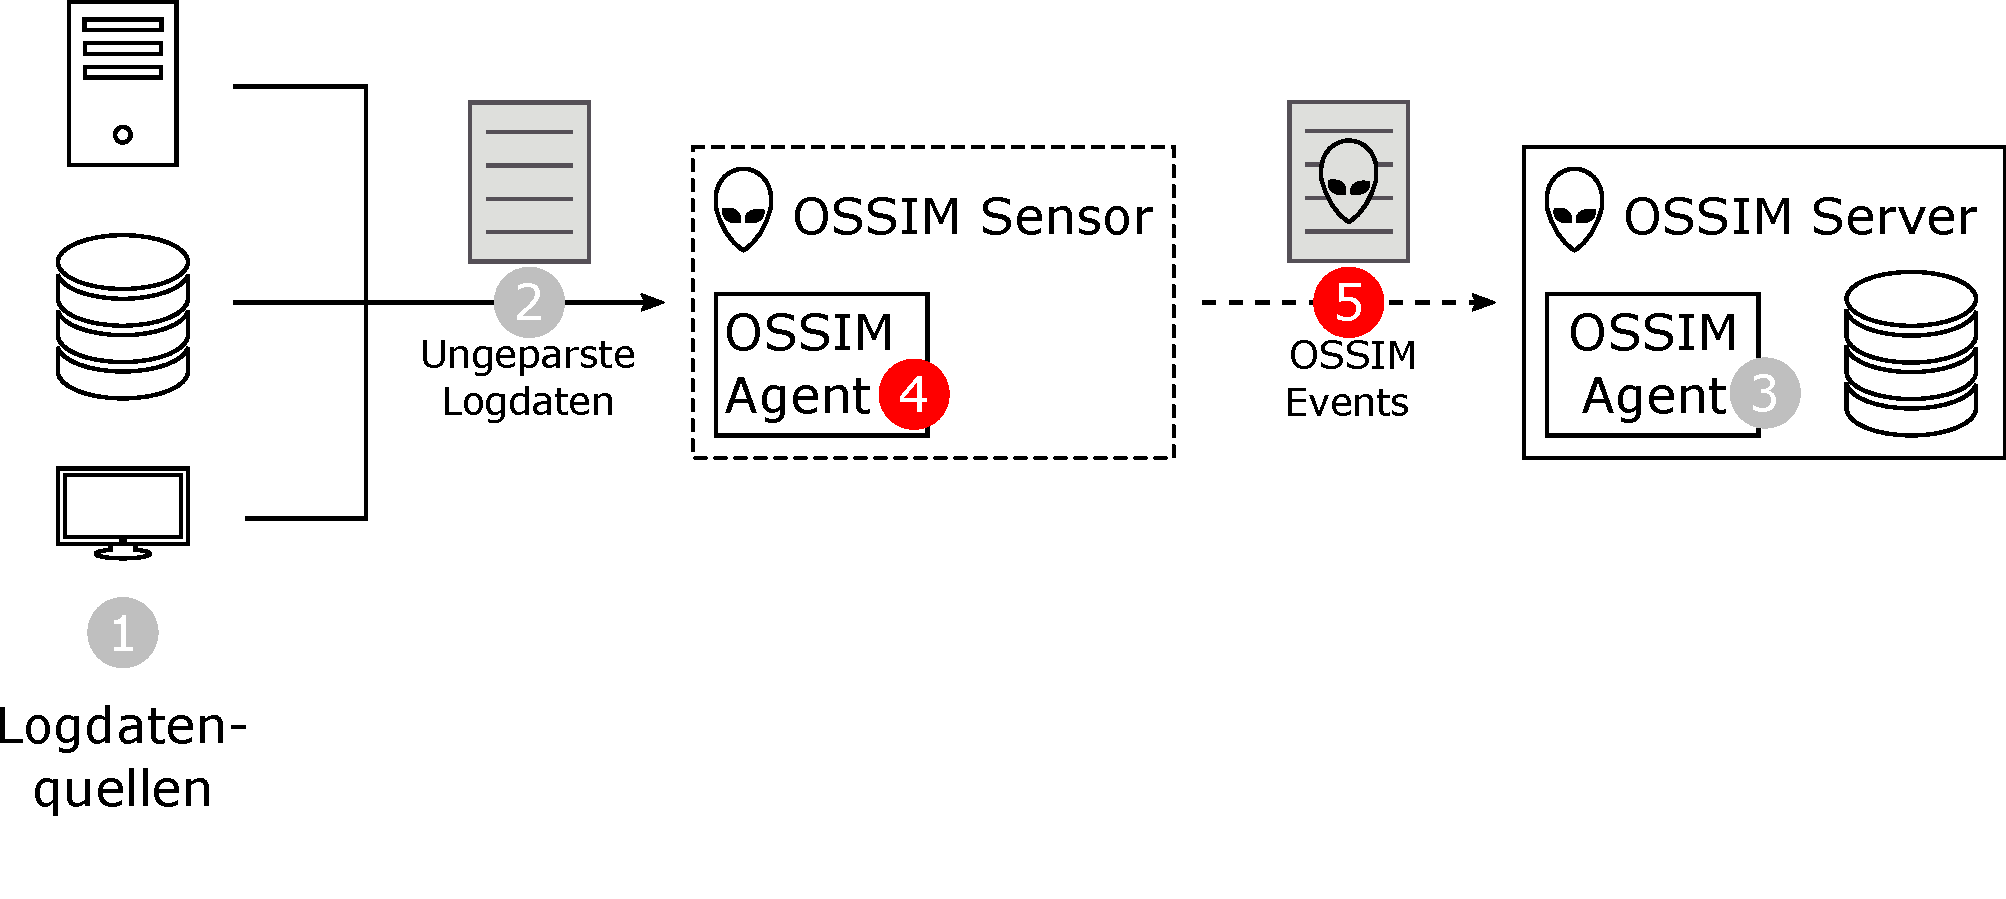
\includegraphics[width=0.9\textwidth]{dia/ossim_data_access_point.pdf}
    \caption{Mögliche Eingriffspunkte in den OSSIM-Datenfluss.}
    \label{fig:ossim_data_access_point}
\end{figure}

Insbesondere der aus datenschutztechnischer Sicht relevante Vorteil, dass die Daten bereits pseudonymisiert in allen OSSIM-Komponenten eintreffen, ließ die Entscheidung auf die \textbf{zweite Möglichkeit} fallen. Dass die Lösung außerdem noch für beide Varianten der OSSIM-Installation möglich ist und keine Anpassungen an OSSIM selbst benötigt, wiegt den Nachteil des zusätzlichen Parsens und wieder Zusammensetzens der Lognachricht bei Weitem auf.\todo{Auch auf Angreifermodell beziehen}





\subsection{Architektur}

%- Beschreibung Architektur
%
%- Wie deckt dieser Ansatz die Anforderungen ab?
%  - Einbindung OSSIM
%  - Pseudonymisierung
%  - Schwellwert
%  - Benutzerinteraktion
%  - Erweiterbarkeit Datenquellen
%  - Erweiterbarkeit Datenschutztechniken

Ausgehend von diesen Überlegungen wurde ein verteiltes System entworfen, dass die Anforderungen aus Abschnitt \ref{sec_impl_requirements} erfüllt und an der beschriebenen Stelle in den Datenfluss eingreift. 
Einen Überblick bietet Abbildung \ref{fig:high__level_architecture}. Das System besteht aus verschiedenen Komponenten, die im Folgenden näher beschrieben werden.

\begin{figure}[]
    \centering
        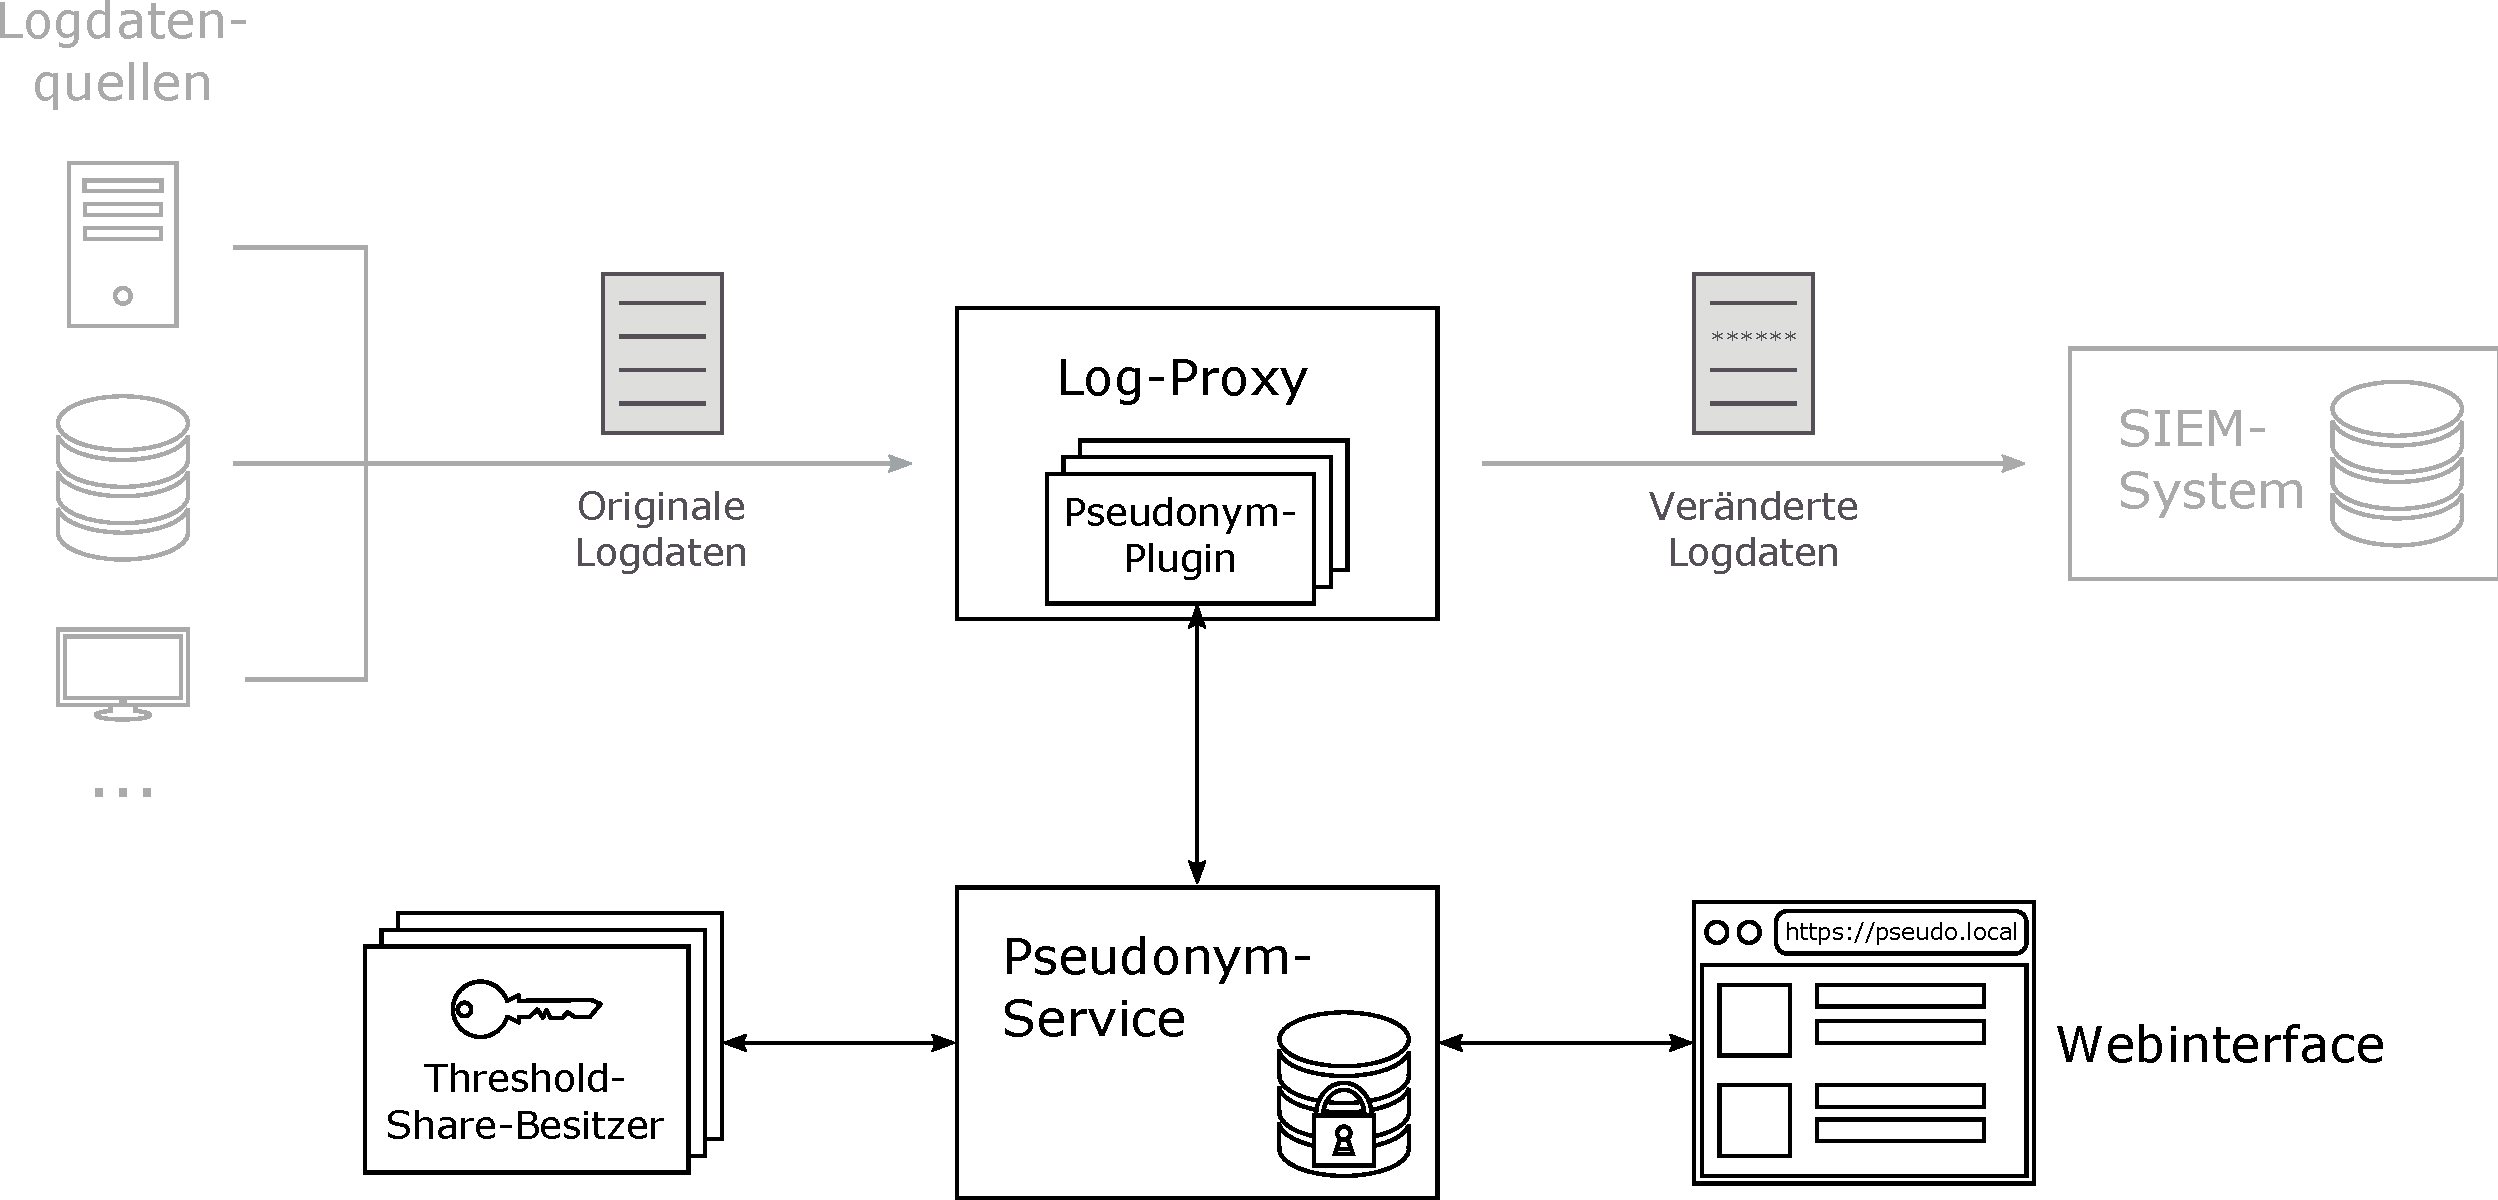
\includegraphics[width=0.9\textwidth]{dia/high_level_architecture.pdf}
    \caption{Ein Überblick über die entworfene Architektur.}
    \label{fig:high__level_architecture}
\end{figure}
\todo{Change Store to Service, Webinterface, Log-Proxy}

Ein \textbf{Log-Proxy}, der die Daten über das Syslog-Protokoll entgegennimmt, verändert und anschließend an OSSIM weiterleitet. Das Verändern der Daten kann mit verschiedenen Plugins geschehen, so dass neben der umzusetzenden Pseudonymisierung auch weitere Datenschutztechniken eingesetzt werden können, was die geforderte Erweiterbarkeit aus Abschnitt \ref{subsec_impl_requirements_plugins} ermöglicht. Der Proxy leistet die Behandlung von Logdaten aus verschiedenen Quellen (siehe Abschnitt \ref{subsec_impl_requirements_differentsources}), was wie bereits im vorhergehenden Abschnitt beschrieben durch Parsen und Wiederzusammensetzen der Daten geschehen muss. Die Konfiguration des quellenabhängigen Vorgehens bei der Logdatenverarbeitung erfolgt ebenfalls hier.

Ein in dem Proxy enhaltenes Plugin wird für die Pseudonymisierung von Daten zuständig und kommuniziert dazu mit einer externen Komponente -- dem Pseudonym-Service. Die Kommunikation mit dem Proxy erfolgt über einen Webservice-basierten Ansatz. Das Plugin kann für eingehende Daten ein Pseudonym anfordern und dieses anschließend in den Logdaten verwenden.

Der \textbf{Pseudonym-Service} erfüllt zwei Aufgaben: das Speichern und Verwalten der Pseudonyme sowie die Integrierung des kryptographischen Schwellwertschemas. Initial muss die Schlüsselgenerierung des Schwellwertschemas (bei zentraler Schlüsselgenerierung) oder die Koordinierung der teilnehmenden Benutzer (bei dezentraler Schlüsselgenerierung) durch den Service geleistet werden. 
Es können während des Betriebs neue Pseudonyme angelegt und zusammen mit ihrem durch das Schwellwertschema verschlüsselten Datum abgelegt werden. Sie werden durch geeignete Maßnahmen durchsuchbar gehalten, um für ein Datum überprüfen zu können, ob bereits ein Pseudonym vergeben wurde. 
Über ein Webinterface kann ein berechtiger Benutzer die Aufdeckung eines bestimmten Pseudonyms fordern und den Status seiner Forderung bzw. im Erfolgsfall das aufgedeckte Datum betrachten. Dieses Datum wird durch das Kombinieren der partiellen Entschlüsselungen erhalten, die von den entsprechenden \textit{Share}-Besitzern berechnet werden.

Benutzer, die zuständig für die Bewertung von Anfragen zur Aufdeckung eines Pseudonyms sind, erhalten die Möglichkeit zur Interaktion mit dem System über eine \textbf{Client-Anwendung}, für die der Pseudonym-Service ebenfalls als Webservice agiert. Diese Anwendungen leisten im Falle der dezentralen Schlüsselgenerierung die initiale Generierung, verwalten den \textit{Share} des Benutzers und können nach der Bestätigung des Benutzers zu der Aufdeckung eines Pseudonyms partiell beitragen. 


\section{Einbindung in OSSIM}

\label{sec_impl_integration_into_ossim}

\subsection*{Ansätze zum Eingriff in den OSSIM-Datenfluss}

\section{Umsetzung der Pseudonymisierung} % und Searchable Encryption

\label{sec_impl_pseudonymity}

% Pseudonymgenerierung

% Parameter: Zeitabhängig, Häufigkeitsabhängig, USE_PFP
% Wie erfolgt die Konfiguration? Wo werden Werte gesetzt/gespeichert?

% MAC Generierung (bzw. Empfang als Search_token) beschreiben

% Zweiter MAC?
% Auch auf Vertrauensmodell im Zusammenhang mit PFP eingehen: Was erfährt die DB, was lässt sich verketten, was würde bei Aufdecken eines Pseudonyms geschehen? Was passiert bei unerlaubtem Zugriff auf gespeicherte Daten?

\todo{Um Implementation erweitern (welche Parameter in welchen Systemteilen, Setup, ...)}

Für die Pseudonymisierung wurde ein Plugin für den Proxy entwickelt, wie in Abschnitt \ref{sec_impl_integration_into_ossim} beschrieben. Bei jedem eintreffenden Logdatum kann abhängig von dem Datenformat für ein entsprechendes Datenfeld ein Pseudonym als Ersatz für das echte Datum gesetzt werden. Dazu stellt der Pseudonym-Service eine Schnittstelle bereit, über die für ein Datum ein Pseudonym erhalten werden kann. Durch diese Trennung wird eine höhere Sicherheit der Zuordnung zwischen Datum und Pseudonym erreicht: In dem Proxy kommen die Logdaten in unveränderter Form an und werden verändert weitergesendet, daher ist die Zuordnung hier implizit bekannt und muss in Kauf genommen werden. Die Speicherung dieser Zuordnung erfolgt jedoch nur in dem Pseudonym-Service. Durch die Verschlüsselung und die in den folgenden Abschnitten beschriebene MAC-abhängige Pseudonymgenerierung erfährt der Pseudonym-Service nichts über das Datum, das durch das Pseudonym beschrieben wird. So führt unberechtigter Zugriff auf die Datenbank des Pseudonym-Service nicht zu mehr Informationen über das Datum, das ein Pseudonym beschreibt.

\subsection{Setup-Phase}

Vor Verwendung der Pseudonymisierung müssen die Parameter zur Pseudonymgenerierung (vgl. Abschnitt \ref{sec_state_pseudonymity}) dem System bekannt gemacht werden. Diese Parameter können in dem Pseudonym-Service mittels einer Konfigurationsoberfläche durch einen berechtigten Benutzer gesetzt werden. Die für den Proxy relevanten Parameter können anschließend über eine Schnittstelle abgefragt werden. Vorerst handelt es sich hierbei lediglich um das maximale Zeitintervall, in dem ein Pseudonym genutzt werden darf.

\subsection{Proxy}

Beim Start des Proxies wird zuerst der gerade beschriebene Parameter erhalten. Anschließend können eintreffende Logdaten verarbeitet werden. Das eintreffende Datum wird verschlüsselt (siehe dazu Abschnitt \ref{sec_impl_threshold}) und anschließend zusammen mit einem über das Datum generierten MAC, der wie in Abschnitt \ref{sec_state_se} beschrieben für die Überprüfung auf bereits bestehende Pseudonyme genutzt wird, an den Pseudonym-Service gesendet. Das ursprüngliche Datum wird nun durch das gelieferte Pseudonym (siehe nächsten Abschnitt) ersetzt und das so veränderte Logdatum wird an das SIEM-System weitergeleitet.

Der Schlüssel, der für die Generierung des MACs verwendet wird, wird abhängig von dem erhaltenen Parameter nach einer bestimmten Zeitspanne neu generiert. Durch diesen Schlüsselwechsel wird wie beschrieben erreicht, das für gleiche Daten, für die der MAC mit einem neuen Schlüssel erstellt wird, auch neue Pseudonyme erhalten werden. 
Da der Schlüsselwechsel nicht Pseudonym-abhängig geschieht, ist die Zeitspanne global für alle Pseudonyme gültig und somit als maximale Zeitspanne zu verstehen. Dies kann für die Anomalieerkennung evtl. Probleme bereiten, wenn nicht genügend lange Überwachungsdaten verkettet werden können. Auf der anderen Seite würde eine Verweildauer für einzelne Pseudonyme ein Erfassen des Erstellungszeitpunkts in der Datenbank erfordern, was wie in Abschnitt \ref{sec_state_pseudonymity} beschrieben Rückschlüsse auf das ursprüngliche Datum des Pseudonyms liefern könnte. Daher wurde sich gegen diesen Ansatz entschieden.

\subsection{Service}

Auf der Service-Seite wird anhand des empfangenen MACs durch Vergleich mit in der Datenbank vorliegenden MACs überprüft, ob bereits ein Pseudonym für das eintreffende Datum vergeben wurde, das noch nicht zu häufig verwendet wurde. Hierzu wird der in der Konfiguration gesetzte Parameter zur maximalen Nutzungshäufigkeit von Pseudonymen verwendet. Liegt kein solches Pseudonym vor, so wird ein noch nicht verwendetes, zufälliges Pseudonym erstellt und zusammen mit dem MAC und dem verschlüsselten Datum in der Datenbank gespeichert. Anderenfalls wird das bereits vergebene Pseudonym zurückgeliefert. 

\subsection{Perfect Forward Privacy}

Im Zusammenspiel dieser Parameter kann jedoch noch ein Problem entstehen. Für neu vergebene Pseudonyme, die innerhalb eines Zeitabschnitts durch Überschreiten der maximalen Nutzungsanzahl entstanden sind, liegen in der Datenbank Einträge mit gleichem MAC vor. Auf diese Weise wird die Verknüpfung verschiedener Pseudonyme ermöglicht, wenn jemand (berechtigt oder unberechtigt) Zugriff auf die Daten erhält. Das Aufdecken eines Pseudonyms deckt auch alle anderen in diesem Zeitintervall erstellten Pseudonyme implizit auf, was dem in Abschnitt \ref{sec_state_pseudonymity} beschriebenen Prinzip der \textit{Perfect Forward Privacy} widerspricht. 

Dieses Problem könnte durch eine Hashwert-Berechnung für den eintreffenden MAC auf der Service-Seite verhindert werden, die einen Pseudonym-abhängigen Zufallswert (eine Art Salt) einbezieht. Hierdurch enthalten Datenbankeinträge, die innerhalb eines Zeitintervalls zu dem gleichen Datum gehören und daher den gleichen MAC besitzen, durch den einfließenden Zufallswert unterschiedliche Hashwerte. Durch die Einweg-Eigenschaft der Hashfunktion wäre die Verkettbarkeit verschiedener Pseudonyme verhindert. 
Jedoch erfordert dieser Ansatz eine Hash-Berechnung pro Datenbankeintrag für jede Anfrage und ist daher aus Performance-Sicht kritisch zu betrachten. Aus diesem Grund wird diese Möglichkeit vorerst nicht implementiert. Das bestehende Problem ist jedoch für ein konkretes Anwendungsszenario und bei der Wahl der Parameter -- insbesondere des Zeitintervalls -- zu beachten.


\section{Implementierung und Integration des Schwellwertschemas}

\label{sec_impl_threshold}

\todo{Einführender Text}

\subsection{ThresholdCrypto \glqq Lib\grqq{}}

%- Bibliothek, die statuslos in allen Teilen des Systems verwendet werden kann.
%
%- Interface

Um die Funktionen des Schwellwertschema unterschiedlichen Systemteilen einfach zur Verfügung zu stellen, wurde eine Bibliothek entwickelt, die in den verschiedenen Komponenten genutzt werden kann. Das öffentliche Interface der Bibliothek stellt folgende Funktionen bereit:

\begin{itemize}
  \item \textbf{Parametergenerierung: } Diese Funktion dient dem Erhalt der benötigten sicheren Primzahl bzw. des Generator (vgl. \todo{ergänzen}). Hierbei kann zwischen Neugenerierung und Verwendung vorberechneter Parameter verschiedener Schlüsselstärken entschieden werden. Näheres dazu ist im Unterabschnitt \textit{Parametegenerierung} zu finden.
  \item \textbf{Schlüssel- und Sharegenerierung: } Durch diese Funktion wird ein zufälliger geheimer Schlüssel erzeugt und aus ihm der öffentliche Schlüssel sowie die einzelnen \textit{Shares} erzeugt. 
  \item \textbf{Verschlüsselung einer Nachricht: } Diese Funktion verschlüsselt mithilfe des öffentlichen Schlüssels eine Nachricht (siehe auch Unterabschnitt \textit{Hybride Kryptographie}). Sie wird im Proxy verwendet.
  \item \textbf{Berechnung einer partiellen Entchlüsselung: } Mithilfe eines \textit{Shares} wird die zugehörige partielle Entschlüsselung einer verschlüsselten Nachricht berechnet. Diese Funktion wird in den Threshold-Clients genutzt.
  \item \textbf{Kombinieren von partiellen Entschlüsselungen: } Aus ausreichend partiellen Entschlüsselungen kann die Nachricht wiederhergestellt bzw. entschlüsselt werden (siehe wiederum Unterabschnitt \textit{Hybride Kryptographie}).
\end{itemize}

Neben den Funktionen werden noch einige Klassen zur Verfügung gestellt, die das Arbeiten mit den Ergebnissen der Funktionen erleichtern sowie Funktionalität wie Serialisierbarkeit ermöglichen:

\begin{itemize}
  \item \textbf{ThresholdParameters: } Enthalten die Werte \(t\) und \(n\) des Schwellwertschemas.
  \item \textbf{KeyParameters: } Enthalten die benötigten Primzahlen bzw. den Generator der zugrundeliegenden Gruppe.
  \item \textbf{PublicKey: } Enthält den öffentlichen Schlüssel der zum Verschlüsseln einer Nachricht verwendet werden kann.
  \item \textbf{KeyShare: } Enthält die Werte des Shares eines Teilnehmers am Schwellwertschema.
  \item \textbf{EncryptedMessage: } Enthält die Daten einer verschlüsselten Nachricht (vgl. auch Abschnitt \ref{sec_impl_threshold_hybrid}).
  \item \textbf{PartialDecryption: } Enthält die zu einer partiellen Entschlüsselung gehörenden Werte, die zum Entschlüsseln der vollständigen Nachricht genutzt werden.
\end{itemize}

Im Folgenden soll kurz auf zwei Kernelemente des implementierten Verfahrens eingegangen werden.

\subsubsection{Parametergenerierung}
  
 \label{sec_impl_threshold_keyparams}
  
%  - Verwendete Gruppen und Auswirkungen fester Parameter? HoC, ...

% https://crypto.stackexchange.com/questions/1451/elgamal-multiplicative-cyclic-group-and-key-generation
% Introduction to modern cryptography 8.3.3 (pdf 343ff)
% Sharing of parameters: Introduction to modern cryptography ElGamal implementation issues (pdf 425)

Die für das Verfahren benötigten sicheren Primzahlen \(p\) und \(q\) lassen sich mithilfe eines einfachen Ansatzes finden \cite{hoc1996}: Es wird solange eine Primzahl \(q\) im Bereich der vorgegebenen Schlüsselstärke zufällig gewählt, bis \(2q + 1\) ebenfalls eine Primzahl ist. Zur Überprüfung der Primalität der entsprechenden Zahlen wird der Miller-Rabin-Test genutzt.\todo{EZ: Miller Rabin ganz kurz erklären}

Zusätzlich benötigt das Verfahren einen Generator \(g\) einer Untergruppe der Ordnung \(q\) von \(\mathbb{Z}_p^*\). Hierzu wird lediglich solange ein zufälliges Element \(g\) aus \(\mathbb{Z}_p^*\) gewählt bis 

\[g^q \equiv 1 \mod p \text{ und } g^2 \not\equiv 1 \mod p\] 

gelten. Da Untergruppen von \(\mathbb{Z}_p^*\) nach dem Satz von Lagrange lediglich die Ordnungen \(1, 2, q\) oder \(2q\) besitzen, werden durch obenstehende Bedingungen lediglich Untergruppen der Ordnung \(q\) zugelassen.

Nach \cite{katz2014} beeinträchtigt es nicht die Sicherheit des ElGamal-Verfahrens, wenn vorberechnete Parameter von verschiedenen Benutzern geteilt werden. Auch die Kombination dieses Verfahrens mit Shamirs Secret Sharing dürfte hieran nichts ändern, da das Secret Sharing lediglich für die Aufteilung des geheimen Schlüssels in Shares sorgt, aber an den grundlegenden Eigenschaften der Ver- und Entschlüsselung im ElGamal-Schema nichts ändert. Daher wurden verschiedene Parameter bereits vorberechnet und als statische Parameter zur Verfügung gestellt. Weiterhin ist es jedoch auch möglich eigene Parameter in gewünschter Stärke zu generieren. \todo{evtl. auf Evaluation beziehen.} In den meisten Empfehlungen werden heutzutage Schlüssellängen um 2000 Bit empfohlen\footnote{
  Für einen Vergleich verschiedener Empfehlungen siehe: https://www.keylength.com
}.

\subsubsection{Hybride Kryptographie}

\label{sec_impl_threshold_hybrid}
  
%  - Erzeugung symmetrischer Schlüssel und symmetrische Kryptographie per NaCl(pynacl) -> Authenticated Encryption ChaCha Salsa
%  
%  - lediglich Verschlüsselung dieses Schlüssels mit dem Schwellwertschema
%  
%  - von erfahrenen Kryptographen entwickelt
%  - getestet
%  - schnell
%  - Beliebiger Nachrichteninhalt ohne Auswirkungen auf die Verschlüsselung

Die Verschlüsselung bzw. Entschlüsselung wurden in Form eines hybriden Verschlüsselungsverfahrens umgesetzt, wie es auch in \cite{katz2014} empfohlen und beschrieben wird: Bei der Verschlüsselung wird ein zufälliger Schlüssel \(k^{symm}\) für ein symmetrisches Verfahren \(E^{symm}\) erzeugt und dazu genutzt den Klartext \(m\) zu verschlüsseln. Das kryptographische Schwellwertschema wird lediglich dazu verwendet, \(k^{symm}\) zu verschlüsseln. Ein Schlüsseltext besteht daher aus drei Teilen: 
\begin{itemize}
  \item \(v = g^k\): Der erste Teil der ElGamal-Verschlüsselung des symmetrischen Schlüssels (siehe Abschnitte \ref{sec_basics_threshold_elgamal} und \ref{sec_state_threshold_scheme})
  \item \(c^{tc} = k^{symm} \cdot g^{ak}\): Der zweite Teil der ElGamal-Verschlüsselung des symmetrischen Schlüssels (siehe Abschnitte \ref{sec_basics_threshold_elgamal} und \ref{sec_state_threshold_scheme})
  \item \(c^{symm} = E^{symm}_{k^{symm}}(m)\): Der symmetrisch verschlüsselte Klartext
\end{itemize}

Bei der Entschlüsselung wird ähnlich vorgegangen: Das kryptographische Schwellwertschema wird dazu genutzt, den symmetrischen Schlüssel wiederherzustellen. Anschließend kann der ursprüngliche Klartext mit diesem Schlüssel wieder entschlüsselt werden. Dieses hybride Vorgehen bietet einige Vorteile: 

Symmetrische Verfahren sind im Allgemeinen deutlich schneller als asymmetrische. Durch die Kombination beider Verfahren wird also erreicht, dass die Eigenschaften des kryptographischen Schwellwertschemas im Bezug auf die verteilte Ver- bzw. Entschlüsselung erhalten werden, jedoch mit dem Geschwindigkeitsvorteil der symmetrischen Verschlüsselung. 

Das Vorgehen ermöglicht es weiterhin beliebige Nachrichten relativ einfach zu verschlüsseln, da die Beschränkung des asymmetrischen Verfahrens bezogen auf die Nachrichtenlänge (die in kodierter Form kleiner sein muss als der Parameter \(p\)) nur noch für den Schlüssel des symmetrischen Verfahrens erfüllt werden muss. Dies stellt kein Problem dar, da symmetrische Verfahren für vergleichbare Sicherheit geringere Schlüssellängen benötigen als asymmetrische Verfahren, die auf dem Diskreten-Logarithmus-Problem beruhen.

Weiterhin kann für die symmetrische Verschlüsselung ein Verfahren genutzt werden, dass neben der Verschlüsselung auch die Validität der Daten überprüft - ein sogenanntes \textit{Authenticated Encryption Scheme}. Hierdurch wird erreicht, dass Änderungen am Schlüsseltext bei der Entschlüsselung erkannt werden und der Vorgang abgebrochen werden kann, also neben der Vertraulichkeit auch die Integrität der Nachricht geschützt ist. 

In der Implementierung wird die Standardfunktion zur symmetrischen Verschlüsselung aus der Kryptographie-Bibliothek NaCl\footnote{
  NaCl: Networking and Cryptography library: https://nacl.cr.yp.to
} 
genutzt. Hierbei handelt es sich um ein \textit{Authenticated Encryption Scheme} auf Basis der Algorithmen Salsa20 und Poly1305. Neben den bereits erwähnten Vorteilen eines hybriden Kryptosystems handelt es sich hierbei zusätzlich um eine weit verbreitete und von erfahrenen Kryptographen entwickelte und überprüfte Bibliothek. Dies erhöht das Vertrauen in eine sichere Umsetzung der Verfahren.

Eine direkte Implementierung des bis hierhin beschriebenen hybriden Schemas enthält jedoch noch eine Schwäche: In \cite{boneh2000} wird von den Autoren ein Angriff vorgestellt, der bei der direkten Implementierung von auf dem ElGamal-Verfahren basierenden Schemata möglich ist. Der Angriff besteht darin, dass bei der Verschlüsselung symmetrischer Schlüssel durch deren geringere Länge und die Berechnungen in speziellen Untergruppen im ElGamal-Verfahren die Möglichkeit besteht, die symmetrischen Schlüssel mit geringerem Aufwand zu entschlüsseln.

Als Gegenmaßnahme wird die Vorverarbeitung der symmetrischen Schlüssel empfohlen. In \cite{abdalla1999} wird ein hybrides Schema dargestellt, dass diese Gegenmaßnahme umsetzt. Der entscheidende Schritt im Vorgehen besteht darin, den symmetrischen Schlüssel nicht direkt zufällig zu erzeugen. Stattdessen wird ein zufälliges Untergruppenelement des Nachrichtenraums \(r \in \mathbb{Z}_q^*\) gewählt und der symmetrische Schlüssel mithilfe einer kryptographisch sicheren Hashfunktion \(H\) hieraus abgeleitet. Hierdurch verändert sich die Zusammensetzung eines Schlüsseltextes leicht:

\begin{itemize}
  \item \(v = g^k\): wie vorhergehend beschrieben
  \item \(c^{tc} = r \cdot g^{ak}\): Anstelle des symmetrischen Schlüssels wird das Untergruppenelement \(r\) durch das ElGamal-Verfahren verschlüsselt.
  \item \(c^{symm} = E^{symm}_{H(r)}(m)\): Als symmetrischer Schlüssel wird nun der durch \(H\) berechnete Hashwert von \(r\) genutzt
\end{itemize}

Zusätzlich schreibt das Schema nach \cite{abdalla1999} die Benutzung eines MACs zur Sicherung der Integrität der Nachricht vor. Auf diesen Schritt kann in dem in dieser Arbeit implementierten Schema verzichtet werden, da die Integrität bereits durch das verwendete AE-Verfahren\todo{EZ: Wird die Abkürzung irgendwo eingeführt?} geschützt ist. Einen Überblick über das letztlich umgesetzte Schema, das auch diesen Angriff verhindert, bietet Abbildung \ref{fig:hybrid_scheme}.

\begin{figure}[]
    \centering
        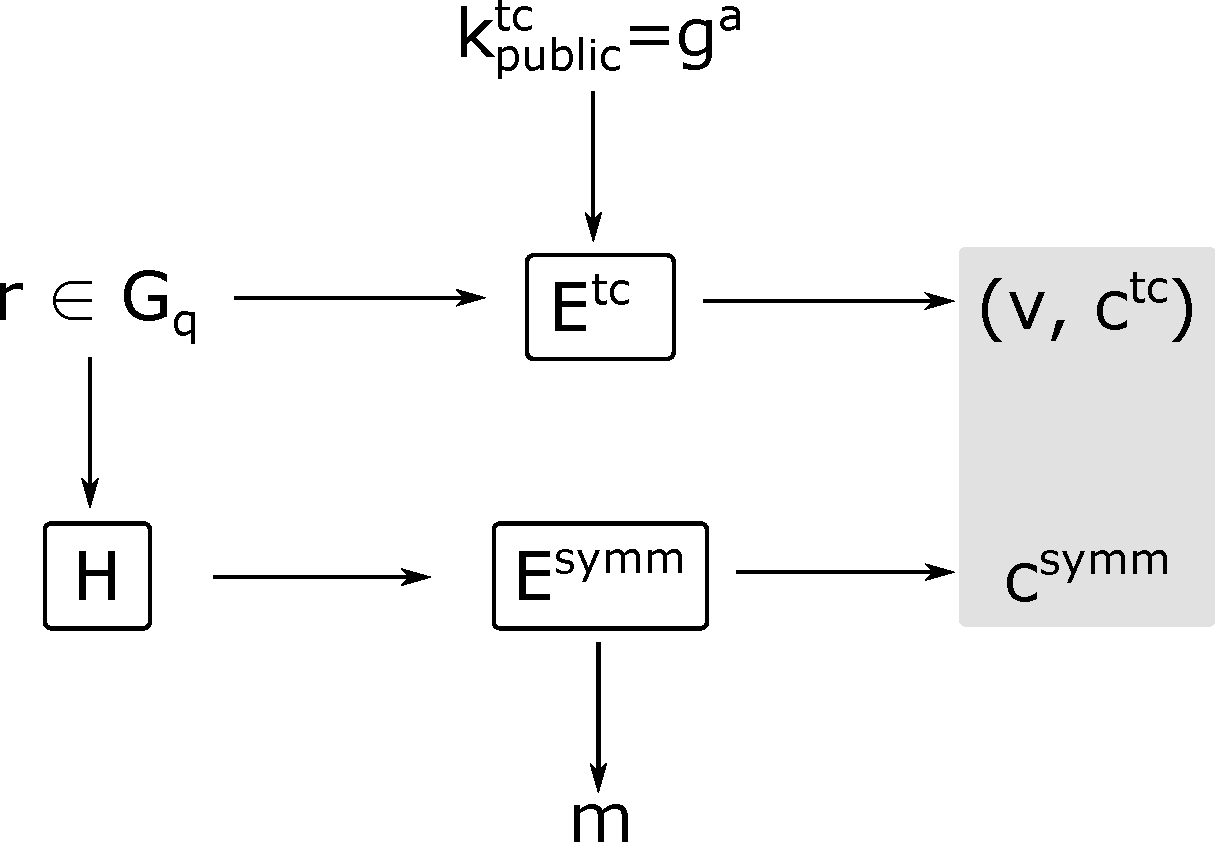
\includegraphics[width=0.4\textwidth]{dia/hybrid_scheme.pdf}
    \caption{Übersicht über das umgesetzte hybride Verschlüsselungsschema.}
    \label{fig:hybrid_scheme}
\end{figure}

\subsection{Service und Setup-Verfahren}

% Setup: Clients, KeyParameter, ThresholdParameter
% auf bereits in impl-pseudonymity geschriebenes zurückgreifen

Um die Parameter für das kryptographische Schwellwertschema setzen zu können, wurde die Konfigurationsoberfläche erweitert. Hier müssen nun Angaben zur Schlüsselstärke, zu beteiligten Teilnehmern und erforderlichen Anzahl an Teilnehmern für die Entschlüsselung eines Datenbankeintrages gemacht werden.

Anschließend können berechtigte Benutzer die Aufdeckung eines Pseudonyms über das Webinterface anfragen. Anschließend werden von den teilnehmenden Clients die partiellen Entschlüsselungen entgegengenommen. Liegen ausreichend partielle Verschlüsselungen vor, so werden diese mithilfe der Bibliothek kombiniert und damit der Halter des Pseudonyms entschlüsselt und aufgedeckt. 

\subsection{Client-Anwendung}

%- Shares empfangen und verschlüsselt abspeichern
%
%- Enthält Webserver um Shares niemals auf dem Server speichern zu müssen

Für Teilnehmer, die an dem Schwellwertschema beteiligt sind, wurde eine konsolenbasierte Anwendung entwickelt, die die folgende Funktionalität bereitstellt:

Clients melden sich zu Beginn an dem Pseudonym-Service an und können in der anschließenden Setup-Phase mit in das Verfahren integriert werden. Jeder teilnehmende Client empfängt nach der Generierung das für ihn bestimmte Share vom Server und speichert dieses verschlüsselt lokal ab. Hierzu enthält die Anwendung einen lokalen Webserver. Dies ermöglicht es dem Pseudonym-Service die \textit{Shares} nicht speichern und nach der Generierung sofort entfernen zu können. 

Anschließend können sich Teilnehmer regelmäßig nach neuen Anfragen zur Aufdeckung eines Pseudonyms erkundigen. Wurde eine neue Anfrage empfangen, so kann der Teilnehmen diese annehmen oder ablehnen. Die Annahme führt zur Berechnung einer partiellen Entschlüsselung mithilfe der Bibliotheksfunktion, die anschließend an den Pseudonym-Service gesendet wird.

\subsection{Proxy}

%- Empfängt PublicKey vom Service und nutzt ihn zur Nachrichtenverschlüsselung

Das im Syslog-Proxy implementierte Plugin zur Pseudonymisierung empfängt während der Initialisierung den während der Schlüsselerzeugung generierten öffentlichen Schlüssel vom Pseudonym-Service. Bei einer eintreffenden Syslog-Nachricht werden die zu pseudonymisierenden Daten mit diesem Schlüssel unter Nutzung der Bibliotheksfunktion verschlüsselt und zusammen mit den bereits in Abschnitt \ref{sec_impl_pseudonymity} beschriebenen weiteren Daten an den Service gesendet.

\section{Evaluation}

\label{sec_impl_evaluation}

Inklusive Problemen, ...














